
There are different software solutions for building computer-vision systems. The software for this work encompasses several interdependent parts: image processing and transmission, data processing, and neural networks.

For \textbf{image processing}, several modules are available (OpenCV \cite{ref36}, Scikit-Image \cite{ref37}, SciPy \cite{ref38}, Pillow \cite{ref39}), of which OpenCV and Scikit-Image were built specifically for machine learning. To solve this task, the OpenCV module was used instead of Scikit-Image, because the former also supports reading video via Gstreamer \cite{ref40}, which allows use of the Nvidia video decoder \cite{ref41} integrated into the Jetson. This saves the CPU when reading the image stream and does so significantly more efficiently, leaving more headroom on the system's CPU for image processing and the computer-vision model's work.

For \textbf{data processing} the Pandas \cite{ref42} module is widely used, providing simple and intuitive commands to analyse and manipulate data. This module performs operations on the CPU, and for extreme data volumes data processing can become time-consuming. In addition to Pandas, several alternative modules have been built that are similarly or marginally better optimised, the closest in operating principle and writing style being cuDF \cite{ref44}. cuDF is essentially most similar to Pandas, but uses the GPU instead of the CPU for data processing, which -- especially when handling large data volumes -- gives a significant time advantage over Pandas, because processing takes place with much greater parallelism than on the CPU. At the time of writing, the Pandas module is in use, because the thesis author has broader experience working with this module. There are later plans to switch to development with cuDF for the purpose of software optimisation.

For \textbf{neural networks} there are several platforms and frameworks: TensorFlow \cite{ref45}, Keras \cite{ref46}, PyTorch \cite{ref47}, Scikit-Learn \cite{ref48}, of which the most popular and widely used are TensorFlow and PyTorch. This work used PyTorch, because compared with TensorFlow, PyTorch's syntax is more Pythonic, which makes it easier to integrate with Python objects and makes error messages easier to understand. The thesis author also has prior experience developing with PyTorch.

\section{Computer-vision neural network model}\label{computer-vision-neural-network-model}

There are several models available for object detection, differing from one another in accuracy, input resolution, size, and speed. Choosing a model means accounting for the system's throughput: more capable systems such as servers can run massive, accurate models in parallel with minimal impact on input-processing speed. Smaller systems such as laptops and embedded systems, by contrast, are better suited to running smaller, faster models.

\begin{longtable}[]{@{}
  >{\raggedright\arraybackslash}p{0.2453\linewidth}
  >{\raggedright\arraybackslash}p{0.2830\linewidth}
  >{\raggedright\arraybackslash}p{0.2170\linewidth}
  >{\raggedright\arraybackslash}p{0.2358\linewidth}@{}}
\caption{Table 4.1.1. Overview of the parameters of the most popular models}\\
\toprule\noalign{}
\endhead
\bottomrule\noalign{}
\endlastfoot
\textbf{Model} & \textbf{Max input (px)} & \textbf{Speed (ms)} & \textbf{Accuracy (mAP)} \\
FasterRCNN \cite{ref49} & 1000x600 & 198 & 73.2 (PASCAL VOC 2007) \\
YOLOv5 \cite{ref50} & 1280x1280 & 26.2 (V100 GPU) & 72.7 (MSCOCO) \\
MobileNet SSD V2 \cite{ref51} & 320x320 & 200 (Google Pixel 1) & 22.2 (MSCOCO) \\
EfficientDet \cite{ref52} & 1536x1536 & 153 (V100 GPU) & 55.1 (MSCOCO) \\
\end{longtable}

For this system, the model had to be chosen with the best accuracy-to-speed ratio in mind. The chosen model also had to be capable of processing information from several video inputs at once (see Table 4.1.1).

The YOLOv5 architecture network was selected to solve the task; it was built by Ultralytics \cite{ref53} as an evolution of YOLOv4 \cite{ref54} and is faster and more accurate than its predecessors. It is also a compact model that is easy to run on embedded systems. The model operates on the single-pass frame-processing philosophy (\emph{You Only Look Once}) -- the image passes through the network only once (unlike other models), and within that single pass object detection and classification happen together, which is why the model's detection operation is also faster (see Figure 4.1.1).

\begin{figure}[H]
\centering
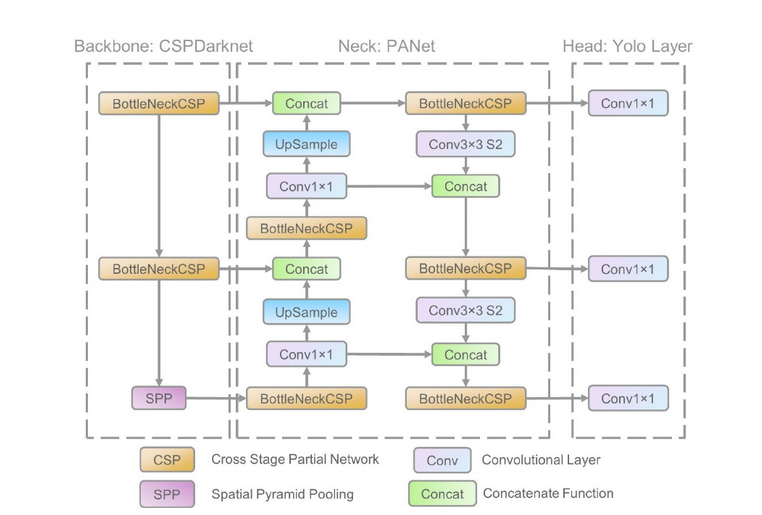
\includegraphics[width=6.10174in,height=4.125in]{media/image12.png}
\caption{Figure 4.1.1. Architecture of the YOLOv5 models \cite{ref55}}
\end{figure}

The model consists of three parts: backbone, neck, and head.

\begin{itemize}
\item
  The \textbf{backbone} is the base on which the model is built; here, CSPNet (\emph{Cross-Stage Partial Network}) was chosen. It is a kind of neural-network model split into several stages (\emph{Cross-Stage}), in which each layer extracts information from the given image -- such as edges and shapes characteristic of the object in the image. Part of the information acquired in earlier layers is passed on to the next layers for processing (\emph{Partial}), which allows the network to progressively understand what the image depicts better and more accurately, using processed information from the previous layers. The backbone consists mainly of convolutional layers and a downsampling layer, whose output passes on to the model's neck. A model with this kind of architecture helps reduce the number of computations required.
\item
  The \textbf{neck} of the neural network is responsible for assembling and organising the information received from the backbone into a feature map, using filters. This model applies a spatial attention pooling method that helps the network focus on important parts of the image, and a Spatial Pyramid Pooling layer, which allows objects to be detected at different resolutions.
\item
  The \textbf{head} generates the probabilities and coordinates of detections for the objects found in the frame. This model also uses anchor boxes, which are pre-configured with given aspect ratios that help detect objects of different sizes and shapes. The model's head contains a number of convolutional layers that predict detection coordinates and probabilities for each object \cite{ref55}.
\end{itemize}
